% CREATED BY DAVID FRISK, 2016
\section{Theory}
In the following the section the underlying theory of the models used in the project are introduced and explained, along with relevant background and examples. 

\subsection{CPG Model}

\subsubsection{Mathematical Model of Physical Behaviour}
%CPG is a mathematical model of human/animal behaviour. Limit cycle, standing wave. Robust, can handle disturbance. (Model different different joints as CPG. Model different DoF as CPG.)

Biological behaviour in mammals, such as walking or swimming, are usually repetative and oscillatory creating energy efficient movements. This can be seen in Figure \ref{fig:walkingCycle}, which shows the walking cycle of a human, measured as the acceleration in Z-direction whilst walking. Due to the rhytmic patterns in the behaviour, it is possible to construct a mathematical model to mimic this type of behaviour. 

\begin{figure}[htbp]
    \centering
    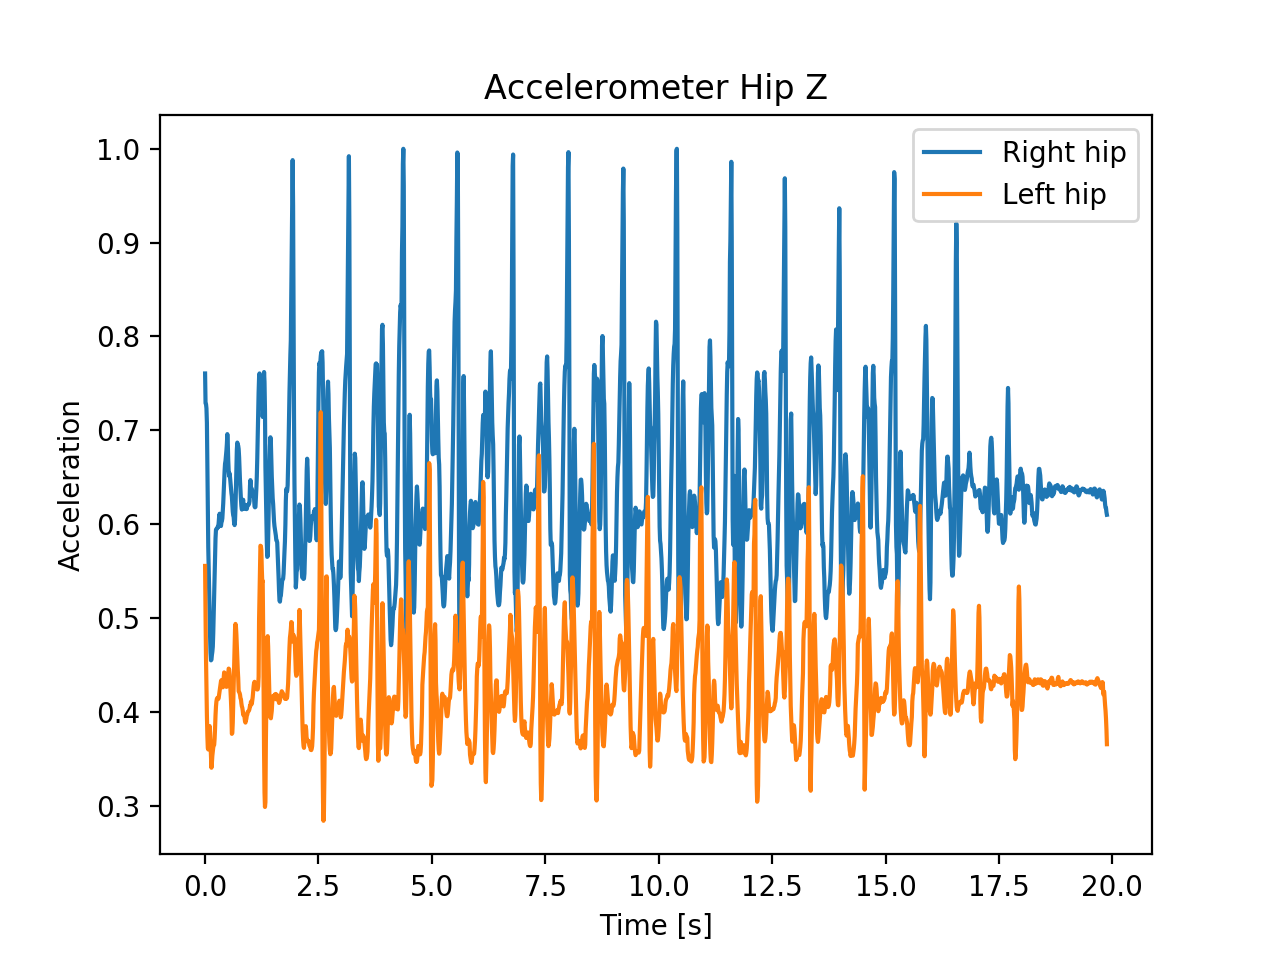
\includegraphics[width=.75\textwidth]{include/figure/reference_right_hip_z.png}
    \caption{Walking cycle of a human. Where \textit{Z} is the horizontal direction of the reference system.}
    \label{fig:walkingCycle}
\end{figure}

A Central Pattern Generator (CPG) is a mathematical model of a neural oscillator, a neural network that produces rhytmic patterned outputs without sensory feedback \cite{CPGHauert}. The output of a CPG can be used as a model of biological rhytmic behaviour, for instance the activation of a certain muscle.

The activity of one muscle in an animal affect the activation of other muscles in its body automatically in order to distribute load and to achieve balance. Similarily CPGs can be modelled as a network, to account for more than a single muscle as well as the interaction between muscles.



\subsubsection{Model of Neural Oscillator} \label{modelOfNeuralOscillator}
%The different existing models. We chose the Matsuoka, show matsuoka sketch, describe parameters.

There exists many different models of CPGs \cite{CPGmodels}, the model to be examined throughout this project is the half-centre model. The half-centre model proposes to account for the alternate activation of the extensor and flexor muscles in the limbs, originally inspired by a cat walking. A mathimatical model was proposed by K. Matsuoka \cite{matsuoka}, using two mutually inhibatory neurons in each oscillator to account for the extensor-flexor behaviour. The model ensures that when one neuron is active, the other is surpressed, creating the oscillatory behaviour.

\begin{figure}[htbp]
    \centering
    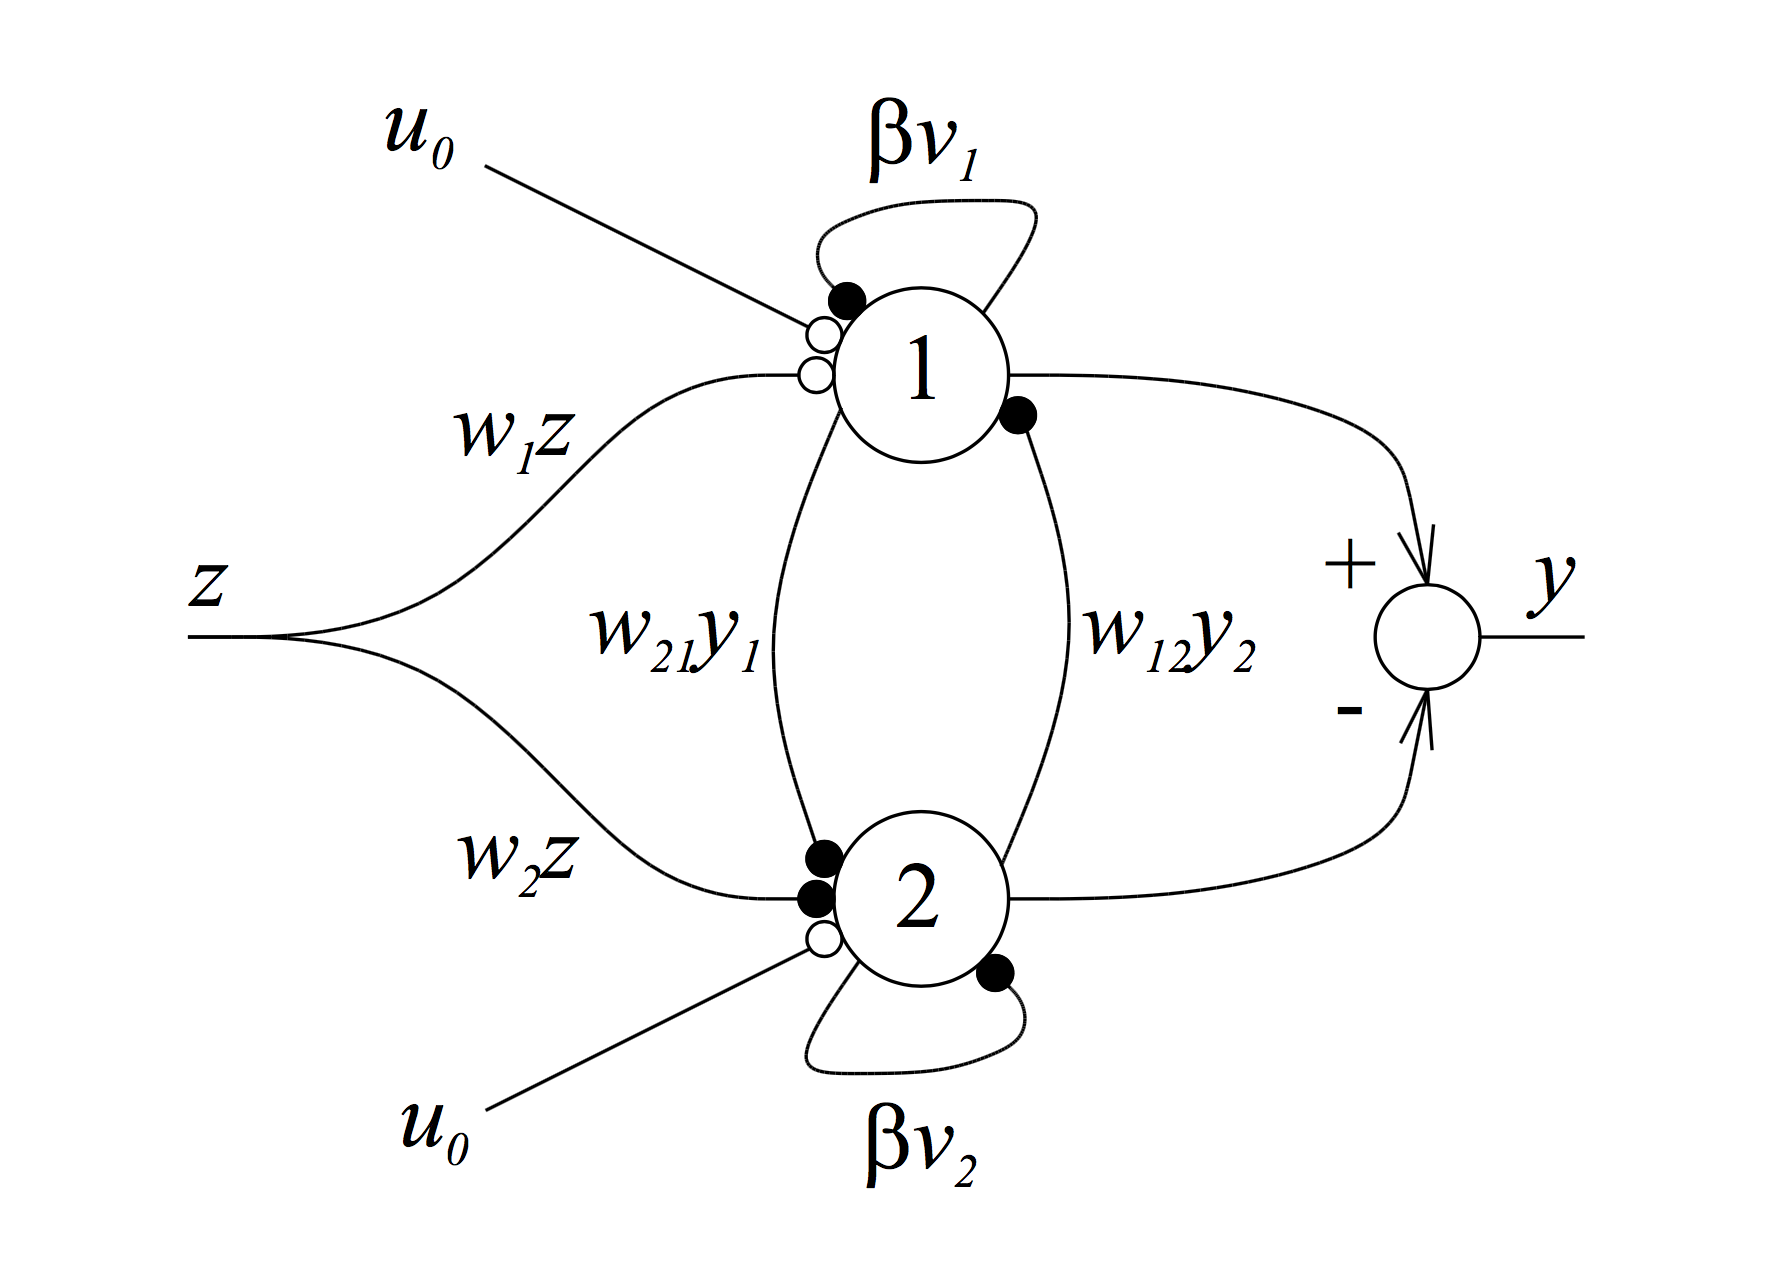
\includegraphics[width=0.75\textwidth]{include/figure/matsuoka.png}
    \caption{The Matsuoka model of a half-centre CPG \cite{CPGwolff}, with parameters explained in Table \ref{tab:parameters}.}
    \label{fig:matsuoka}
\end{figure}

The setup of the Matsuoka model is shown in Figure \ref{fig:matsuoka}, with the parameters as described in Table \ref{tab:parameters}. The behaviour of the model is described by the following equations \cite{CPGequations}:

\begin{align}
    \tau_u \dot{u}_i &= -u_i - \beta v_i + \sum^{n}_{j=1} w_{ij}y_j + u_0, \\
    \tau_v \dot{v_i} &= -v_i + y_i, \\
    y_i &= \text{max}(0, u_i), \\
    o &= y_2 - y_1
\end{align}

where the model is simulated by integrating over time using Euler integration and timestep $\Delta t$ and $\dot{u}_i$, $\dot{v}_i$ from above in:

\begin{align}
    u_i(t + \Delta t) &= u_i(t) + \Delta t \dot{u}_i, \\
    v_i(t + \Delta t) &= v_i(t) + \Delta t \dot{v}_i.
\end{align}

\begin{table}[htbp]
    \centering
    \begin{tabular}{|c|p{6.5cm}|c|c|}
         \hline
\textbf{Parameter} & \textbf{Description} & \textbf{Initial value} & \textbf{Comment} \\ \hline
$z_i$ & input of neuron i &  & oscillating  \\ \hline
$u_0$ & external tonic input & 1.0 &  \\ \hline
$u_1$ & inner state of neuron 1 & 0.0 & fixed \\ \hline
$u_2$ & inner state of neuron 2 & 1.0 & fixed \\ \hline
$v_1$ & auxiliary variable measuring the degree of self-inhibition of neuron 1 & 1.0 & fixed \\ \hline
$v_2$ & auxiliary variable measuring the degree of self-inhibition of neuron 2 & 0.0 & fixed \\ \hline
$\beta$ & modulation parameter & 2.5 &  \\ \hline
$w_{ij}$ & weights connecting neuron j to neuron i & -2.0 &  \\ \hline
$y_i$ & the output of neuron i & 0 & \\ \hline
$\tau_u$ & time constant & 0.025 &  \\ \hline
$\tau_v$ & time constant & 0.3 &  \\ \hline
$o$ & the output of the oscillator & & \\ \hline
    \end{tabular}
    \caption{The parameters used in the Matsuoka model of a half-centre CPG.}
    \label{tab:parameters}
\end{table}


\subsubsection{Model of CPG Network} \label{CPGnetwork}
%Combining different CPG neurons on a network to model a human where each Neuron is a DoF.

Coupling multiple CPGs into a network makes it possible to model more complex structures, such as an animal or a human. This can be done by connecting the output of one neuron to the input of another. This project investigatex the walking behaviour of a human implemented on a humanoid robot, thus human behaviour can be modelled by looking at the movement in different joints of the body, corresponding to the joints of the humanoid robot. Since the output of a CPG is one-dimensional over time, and human movement is three dimensional, one can imagine modelling the movement in each dimension with a separate CPG. The output signals can then be superimposed to obtain the total movement.


\subsubsection{Choice of Input to Oscillator} \label{choiseOfInputToOscillator}
%The different models (summing output and weights). Asyncronous vs syncronous.
%2.1.3 in old report
Each of the neurons in a CPG network have inputs ($z_i$) that are affected by the output of the other neurons ($o$). One can imagine that all neurons are fully connected, but by setting the weight between two neurons to zero, that weight is \textit{removed}. The input to the neurons can be calculated in different ways, one way inspired by Liu et.al. \cite{liu} is to define the inputs to neuron $i$ as
\begin{align}
z_1 &= \sum_{j \text{ neighbour of } i} a_{ij}u_j, \\
z_2 &= 0.
\end{align}
Another implementation inspired by Shan et.al. \cite{shan} defines the inputs as
\begin{align}
z_1 &= \sum_{j \text{ neighbour of } i} a_{ij}[y_j]^+, \\
z_2 &= \sum_{j \text{ neighbour of } i} a_{ij}[y_j]^-,
\end{align}
where 
\begin{align}
[y_j]^+ &:= \text{max}(y_j,0), \\
[y_j]^- &:= \text{min}(y_j,0).
\end{align}

Neurons can also be affected by an external tonic input ($u_0$). The amplitude of the oscillation in the CPG is proportional to the tonic input. If the input is oscillatory, the oscillator will lock to the frequency of the input. When the input is removed, the oscillator will smoothly return to the original frequency \cite{CPGwolff}.


\subsection{Optimisation Using Genetic Algorithm}
A CPG alone might not achieve satisfactory results, as the parameters in the CPG or network might need to be tweaked and optimised to achieve the desired behaviour. A commonly used technique for optimising behaviour is to use reinforcement learning to improve the model based on an external measure of success. This project uses a Genetic algorithm (GA) as a reinforcement learning technique to achieve desired walking behaviour. A genetic algorithm is an evoutionary algorithm that takes inspration from natural selection implemented as an optimisation problem \cite{GAHauert}. 


\subsubsection{Genome}
%Difference between using only weights or the entire CPG network as genome.


The \textit{genome} is a set of parameters that defines a proposed solution to the problem that the GA is trying to solve. One can imagine various different genomes when optimising the behaviour of a CPG, for instance the internal parameters in the CPG, shown in Table \ref{tab:parameters}. The connection weights between neurons in a CPG network, as described in Section \ref{CPGnetwork}, could also be used to account relation between CPGs in a network.

\subsubsection{Operators}
%Init population, simulate behaviour, evaluation, selection, mutation, permutation
The basic implementation of a GA is in summary; initialise the population, simulate the behaviour, evaluate success, selecion process, mutation and permutations, repeat until converge. A more detailed description can be found in \cite{wahde}. The evaluation process, also known as the \textit{fitness function}, produces a fitness score which is the measurement the success of the individual. Since this project investigates walking behaviour in a humanoid robot, a fitness function may include e.g.; distance walked, time walked, stability, falling, walking style, etc.